\DiaryEntry{Linear Block Codes}{2017-03-27}{Coding}


\subsection{Definition}

An $(n,k)$ binary block code $\Cc$ is a set of $2^k$ n-vectors called code words. An enocder maps a messsage $m$ (a length-k binary word) to the associated code word $c$.

A \emph{linear} code is a code where the $k$ code words form a $k$-dimensional vector subspace of the vector space of all length-$n$ binary words. In other words, the linear combination of two (or more) codewords is again a codeword.

$n$ is said to be the length of the Code and $R=k/n$ is the code rate.

The Hamming weight $wt(c)$ of a codeword is the number of ones of a codeword $c$. The minimum weight of a code $\Cc$ is the smallest Hamming weight of any non-zero codeword. For a linear code, the minimum distance equals the minimum weight.


\subsection{Generator Matrix Description}

Since a linear block code is a $k$-dimensional vector space, there exists a base of $k$ independent vectors $g_0, g_1,\ldots,g_{k-1}$ for this vector space. Every codeword $c$ can then be represented as linear combination according to

\bee
c = m_0 g_0 + \cdots + m_{k-1} g_{k-1}
\eee
%
In coding, we represent vectors as row vectors; collecting the set of basis vectors in a matrix yields the matrix $G$

\bee
G = \begin{bmatrix} g_0 \\ g_1 \\ \cdots \\ g_{k-1} \end{bmatrix}
\eee
%
Collecting the message into a length-$k$ vector $m = [m_0 \cdots m_{k-1}]$ we can write the encoding operations as

\bee
c = m G
\eee
%
In case of a systematic code, the message bits $m_0 ... m_{k-1}$ can be found unchanged in the encoded message $c$; typically, the last $k-1$ elements of $c$ contain the message bits. Note that a code need not be linear; being systematic is a general characterisitc of any code.

For such a systematic linear block code, we can write the matrix $G$ as $G=[P I_k]$, with the matrix $P$ generating the parity check bits and the $k\times k$ identity matrix. The encoding oeration then becomes

\bee
c = mG = m [P I_k] = [mP m]
\eee
%
which shows that the message bits are located at the end of the codeword. 


\subsection{Parity Check Matrix}

The dual code $\Cc^\star$ of a code $\Cc$ is an $(n, n-k)$ code. The $n-k+1$-dimensional basis for the corresponding vector space is the set of vectors $h_0, h_1, \ldots, h_{n-k+1}$ which we again collect in a matrix $H$

\bee
H = \begin{bmatrix} h_0 \\ h_1 \\ \cdots \\ h_{n-k+1} \end{bmatrix}
\eee
%
which is called the parity check matrix. The generator matrix $G$ and the parity check matrix $H$ are connected via

\bee
GH^T = 0
\eee
%
A vector $v$ is a codeword of a code $\Cc$, iff

\bee
vH^T = 0
\eee
%
In case of a systematic linear code, the parity check matrix is given by

\bee
H = [I_{n-k} -P^T] = [I_{n-k} P^T]
\eee


\subsection{Decoding}

\subsubsection{Syndrome}

The syndrome $s$ is calculated via $s = rH^T$ and we have $s=0$ iff $c \in \Cc$.

Assume we transmit the codeword $c = mG$ across a faulty channel which introduces random faults $e$ and receive

\bee
r = c + e
\eee
%
Then the syndrome becomes

\bee
s = (c+e)H^T = cH^T + eH^T = eH^T
\eee


\subsubsection{The Standard Array}

For maximum likelihood decoding, we need to perform the following operation

\bee
\hat{c} = \arg \min_{c \in \Cc} d_H(c,r)
\eee
%
i.e. we choose the codeword being closest (in terms of Hamming distance) to the received word $r$.
%
Let the set of codewords be $\{c_0, c_1,\ldots\}$ and let $V_i$ denote the set of codewords closer to $c_i$ than any other codeword. Vectors having the same distance to more than one codeword are assigned at random to any $V_i$. The sets $V-i$ partition the space of length-n words into $2^k$ disjoint subsets. ML decoding can be alternatively interpreted as determining the set $V_i$ a received word falls into.

The standard array is a representation of this partitioning. It is a table, with the $2^k$ codewords on top. The words of the set $V-i$ are then contained in the $i$-th column. The standard array can be obtained as follows:

\begin{itemize}

\item Write down all codewords as the first row of the array.

\item From the remaining \emph{unused} words, select one with minimum weight and write it into the first column (the column with the all-zero codeword on top). Add the word to the codewords of all other columns.

\item Repeat word selection and proceed as above until all words have been used. 

\end{itemize}


\subsection{Example}

Consider the generator matrix for a $(7,3)$ code

\bee
G = \begin{bmatrix} 0 &1 &1 &1 &1 &0 &0\\
                    1 &0 &1 &1 &0 &1 &0 \\
                    1 &1 &0 &1 &0 &0 &1 \end{bmatrix}
\eee

As outlined above, we will first obtain the codewords by iterating over all $2^3$ message words. Message $[0 0 0]$ yields $[0 0 0 0 0 0 0]$, message $[0 0 1]$ yields $[1 1 0 1 0 0 1]$ and so on.

Let's write the message words and the corresponding codewords into a table like this (we take the MSB to be on the righmost position!!)

\bee
\begin {array}{ccccccccc}
& 000     & 100     & 010     & 110     & 001     & 101     & 011     & 111 \\
& 0000000 & 0111100 & 1011010 & 1100110 & 1101001 & 1010101 & 0110011 & 0001111
\end{array}
\eee

An unused codeword of weight 1 is $[10000000]$; when we add it to the second row (which contains the codewords), we obtain

\bee
\begin{array}{ccccccccc}
         & 000     & 100     & 010     & 110     & 001     & 101     & 011     & 111 \\
         & 0000000 & 0111100 & 1011010 & 1100110 & 1101001 & 1010101 & 0110011 & 0001111 \\
10000000 & 1000000 & 1111100 & 0011010 & 0100110 & 0101001 & 0010101 & 1110011 & 1001111
\end{array}
\eee

We can continue like this and obtain a table like the following. 

\begin{figure}[htb]
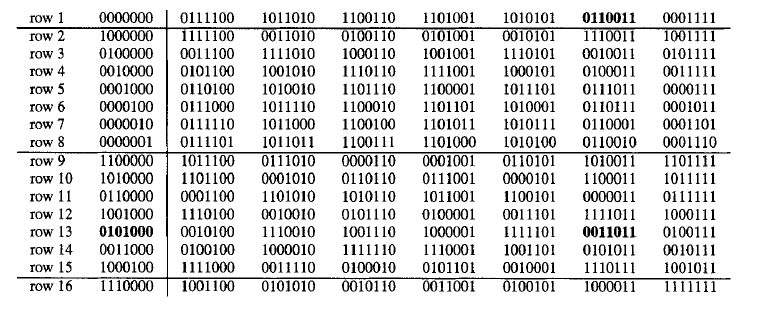
\includegraphics[scale=0.8]{images/standard_array.png}
\end{figure}

From the table we make the following observations:

\begin{itemize}

\item The difference or sum of two words in the same row is a codeword because $(c_i + e_k) \pm (c_j + e_k) = c_i + c_j$ and the sum / difference of two codewords is again a codeword.

\item The words in the same row are all different; If we had $c_i + e = c_j + e$, $c_i = c_j$ would follow which is impossible.

\item The rows of the standard array are cosets as each row is of the form $e + \Cc = \{e + c: c \in \Cc\}$ and the elements in the first column are called coset leaders.

\item The minimum weight of the codewords is $4$ bits.

\item All $1$-bit errors can be corected, $7$ $2$-bit errors can be corrected, and one $3$-bit error can be corrected.

\end{itemize}


\subsection{Syndrome Decoding}

Decoding by means of the standard array is complicated as the table soon becomes infeasibly big. Syndrome decoding is simpler.

It is based on the observation that - for a given error word $e$ - the syndrome does \emph{not} depend on the sent codeword; i.e.

\bee
s = rH^T = eH^T
\eee
%
Syndrome decoding works with a precalculated mapping between syndrome and error word. For every possible syndrome, the error word is calculated. In case several error patterns lead to the same syndrome (this is possible as there are $2^n$ error patterns and only $2^k$ syndromes), the minimum weight error word is taken. 

When a (possibly wrong) codeword is received, the decoder calculates the syndrome. If it is zero, the decoder passes on the received codeword; otherwiese, the decoder looks up the corresponding error pattern, adds the pattern to the received codeword and passes on the result. In any case, a subsequent stage extracts the message bits from the codeword (simple in case of a systematic code).

Continuing the example above, consider the syndrome $[1 1 0 1]$. It is caused by the follwing error patterns: $[0,1,1,0,0,1,0]$, $[1,1,0,0,1,1,1]$, $[1,1,0,1,0,0,0]$, $[1,0,1,1,0,1,1]$, $[0,1,1,1,1,0,1]$, $[0,0,0,0,0,0,1]$, $[0,0,0,1,1,1,0]$, $[1,0,1,0,1,0,0]$. By the description above, the associated error pattern in the syndrome decoding table will be $[0,0,0,0,0,0,1]$; i.e. the error pattern with lowest weight.


